\chapter[Metodologia]{Metodologia}

\section{Gerenciamento}

\subsection{Termo de Abertura do Projeto (TAP)}

O termo de abertura do projeto é essencial para que se documente de forma clara o atual cenário e o que será realizado no projeto, bem como ter noção de planejamento quanto a prazo e custos. O termo de abertura do projeto referente a esse trabalho se encontra disponível no anexo A.

\subsection{Estrutura Analítica do Projeto (EAP)}

A estrutura analítica do projeto possibilita uma visão geral das atividades que serão realizadas ao longo do projeto. Dessa forma, a EAP deste trabalho foi elaborada levando em conta os prazos de entregas, e a separação das macro atividades, ou subsistemas, e das micro atividades. Ela está disponível abaixo:

\begin{figure}[h]
	\centering
	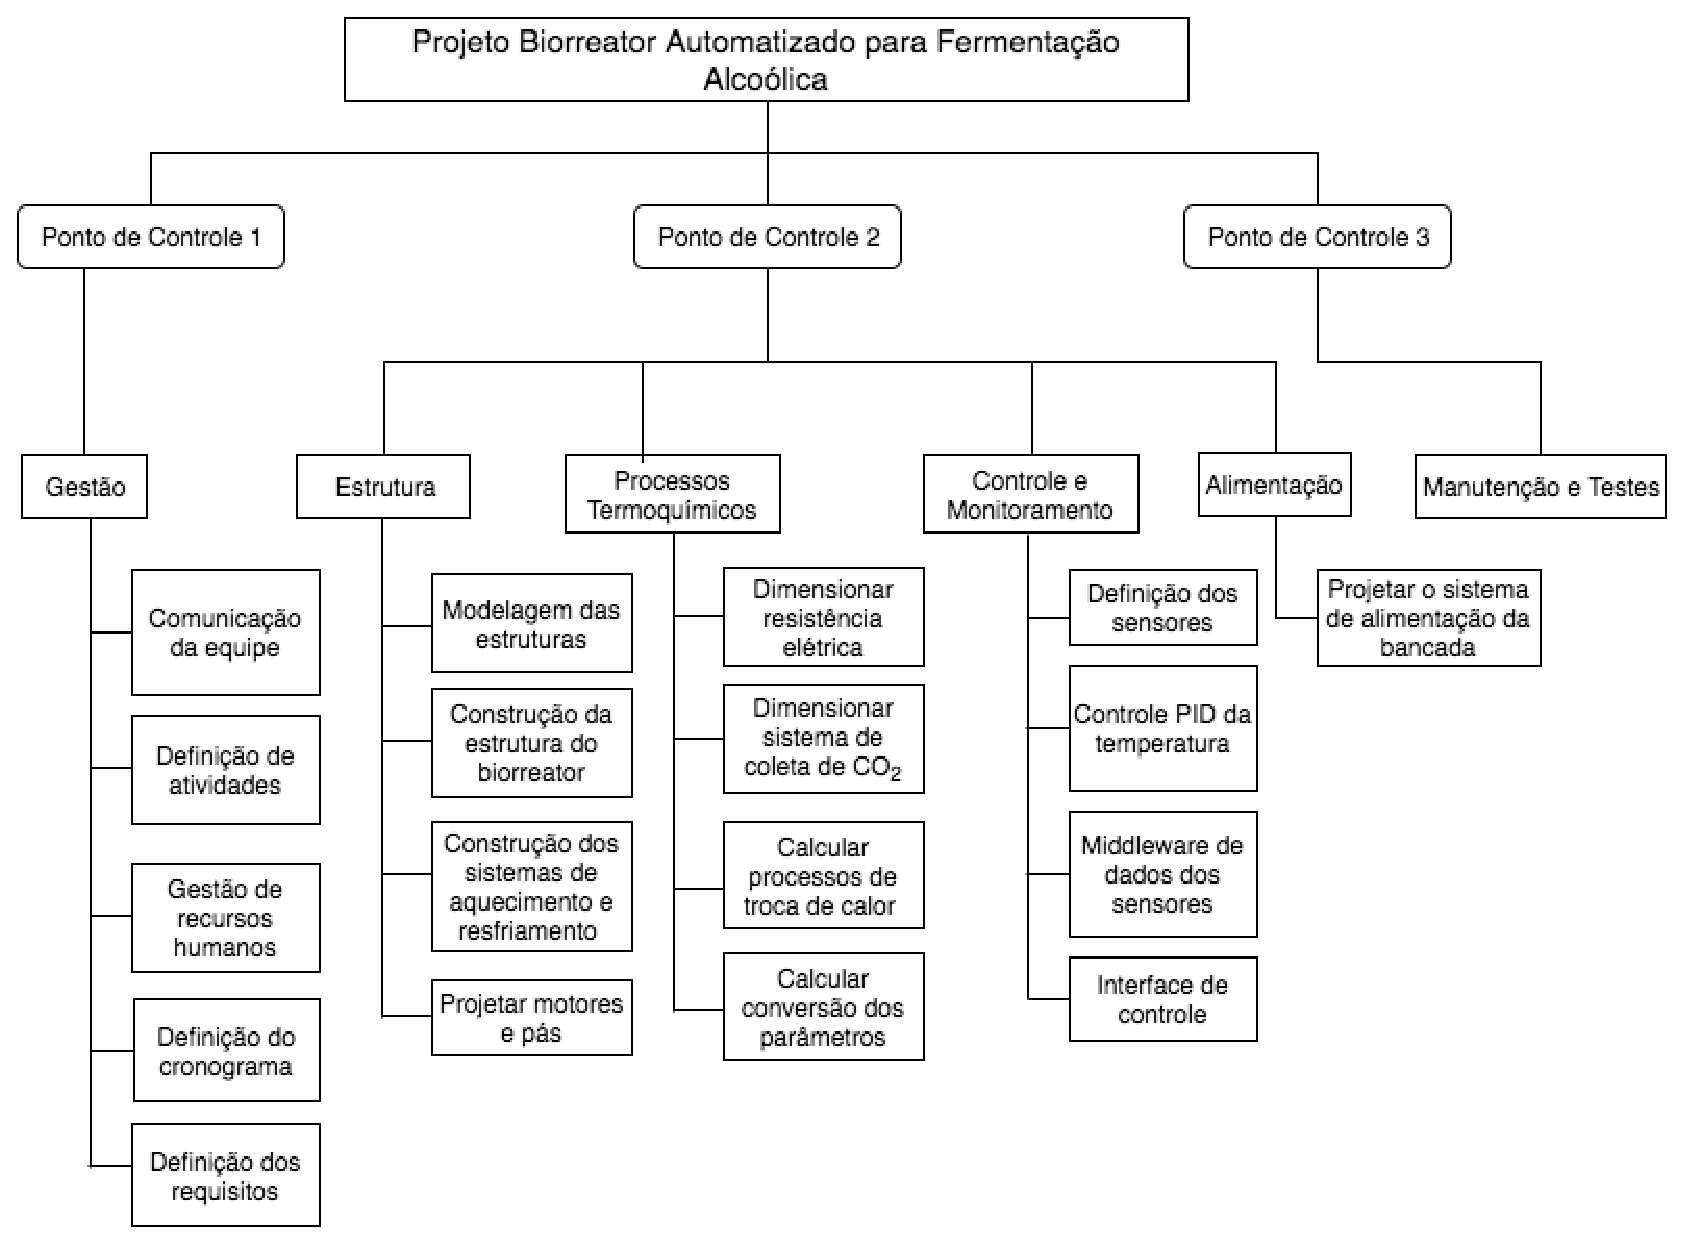
\includegraphics[keepaspectratio=true,scale=0.8, width=\textwidth]{figuras/eap.eps}
	\caption{Estrutura Analítica do Projeto}
	\label{eap}
\end{figure}

\subsection{Tempo}

Baseado nos prazos de entrega nos pontos de controle, foi feito o seguinte cronograma de atividades:

\subsection{Custos}

O gerenciamento dos custos do projeto inclui os processos envolvidos em planejamento, estimativas, orçamentos, financiamentos, gerenciamento e controle dos custos, de modo que o projeto possa ser terminado dentro do orçamento aprovado possuindo foco no custo dos recursos necessários para completar as atividades do projeto.

O gerenciamento dos custos projeto deve considerar também o efeito das decisões de projeto no custo recorrente subsequente do uso, manutenção e suporte do produto, serviço ou resultado do projeto, neste caso ficando limitado a opção da equipe quanto a continuar disponibilizando e oferecendo suporte ao produto final.

A tabela abaixo representa os custos estimados dos materiais selecionados para o desenvolvimento do projeto:

\begin{table}[h]
\centering
\caption{Tabela de custos do projeto}
\resizebox{\textwidth}{!} {
\label{table1}
\begin{tabular}{ll|l|}
\hline
\multicolumn{1}{|l|}{Area}                     & Material                                                                                    & Custo              \\ \hline
\multicolumn{1}{|l|}{ESTRUTURA}                & Conformação mecânica (calandragem) cilíndrica, cônica para aço inoxidável e flange (1,5 mm) & R\$332,00          \\ \hline
\multicolumn{1}{|l|}{}                         & Soldagem inox                                                                               & R\$300,00          \\ \hline
\multicolumn{1}{|l|}{}                         & Tubo de Suporte                                                                             & R\$130,00          \\ \hline
\multicolumn{1}{|l|}{}                         & Tampa flangeada (3 mm)                                                                      & R\$ 120,00         \\ \hline
\multicolumn{1}{|l|}{}                         & Válvula de alívio de pressão                                                                & R\$ 11,15          \\ \hline
\multicolumn{1}{|l|}{}                         & Manômetro                                                                                   & R\$ 37,00          \\ \hline
\multicolumn{1}{|l|}{}                         & 11 Anéis de vedação em silicone (espude)                                                    & R\$ 20,00          \\ \hline
\multicolumn{1}{|l|}{}                         & 2 Torneiras                                                                                 & R\$ 20,00          \\ \hline
\multicolumn{1}{|l|}{}                         & Rotor e Pás                                                                                 & R\$ 50,00          \\ \hline
\multicolumn{1}{|l|}{}                         & Motor                                                                                       & R\$ 300,00         \\ \hline
\multicolumn{1}{|l|}{}                         & Rolamentos                                                                                  & R\$ 10,00          \\ \hline
\multicolumn{1}{|l|}{CONTROLE E MONITORAMENTO} & Sensor Ultrassônico HC-SR04                                                                 & R\$ 15,00          \\ \hline
\multicolumn{1}{|l|}{}                         & 2 Sensores DS18B20 para temperatura                                                         & R\$ 20,40          \\ \hline
\multicolumn{1}{|l|}{}                         & 2 sensores MPX5700DP                                                                        & R\$ 123,00         \\ \hline
\multicolumn{1}{|l|}{}                         & Gravity Analog pH Meter Kit                                                                 & R\$ 147,00         \\ \hline
\multicolumn{1}{|l|}{}                         & Motor de Passo 28BYJ-48 + Driver ULN2003                                                    & R\$ 20,00          \\ \hline
\multicolumn{1}{|l|}{}                         & Conversor A/D ADS1115                                                                       & R\$ 24,00          \\ \hline
\multicolumn{1}{|l|}{}                         & Raspberry PI 3                                                                              & R\$ 200,00         \\ \hline
\multicolumn{1}{|l|}{PROCESSOS TERMOQUÍMICOS}  & Resistência elétrica 5000 W 220 V                                                           & R\$ 100,00         \\ \hline
\multicolumn{1}{|l|}{}                         & Bomba de circulação 220 V                                                                   & R\$ 250,00         \\ \hline
\multicolumn{1}{|l|}{}                         & Mangueira de silicone                                                                       & R\$ 14,00/m        \\ \hline
\multicolumn{1}{|l|}{}                         & Alga chaetomorpha                                                                           & R\$ 34,90          \\ \hline
\multicolumn{1}{|l|}{}                         & Válvula de esfera para gás borboleta fêmea                                                  & R\$ 30,00          \\ \hline
\multicolumn{1}{|l|}{ALIMENTAÇÃO}              & Cabo de Força 3m                                                                            & R\$ 25,00          \\ \hline
                                               &                                                                                             & TOTAL: R\$2.419,55 \\ \cline{3-3}
\end{tabular}
}
\end{table}

\subsection{Alocação de recursos humanos}

A equipe do projeto é formada por 12 membros que foram divididos de acordo com as macro atividades que serão realizadas. Em cada uma delas foi escolhido um membro líder responsável pela supervisão das atividades. Além disso, foi escolhido um líder geral, o gerente do projeto, responsável pela integração de todas as partes do mesmo, e um outro gerente responsável pelo controle de qualidade das atividades. Abaixo se tem a relação esquemática da divisão adotada.

\begin{figure}[h]
	\centering
	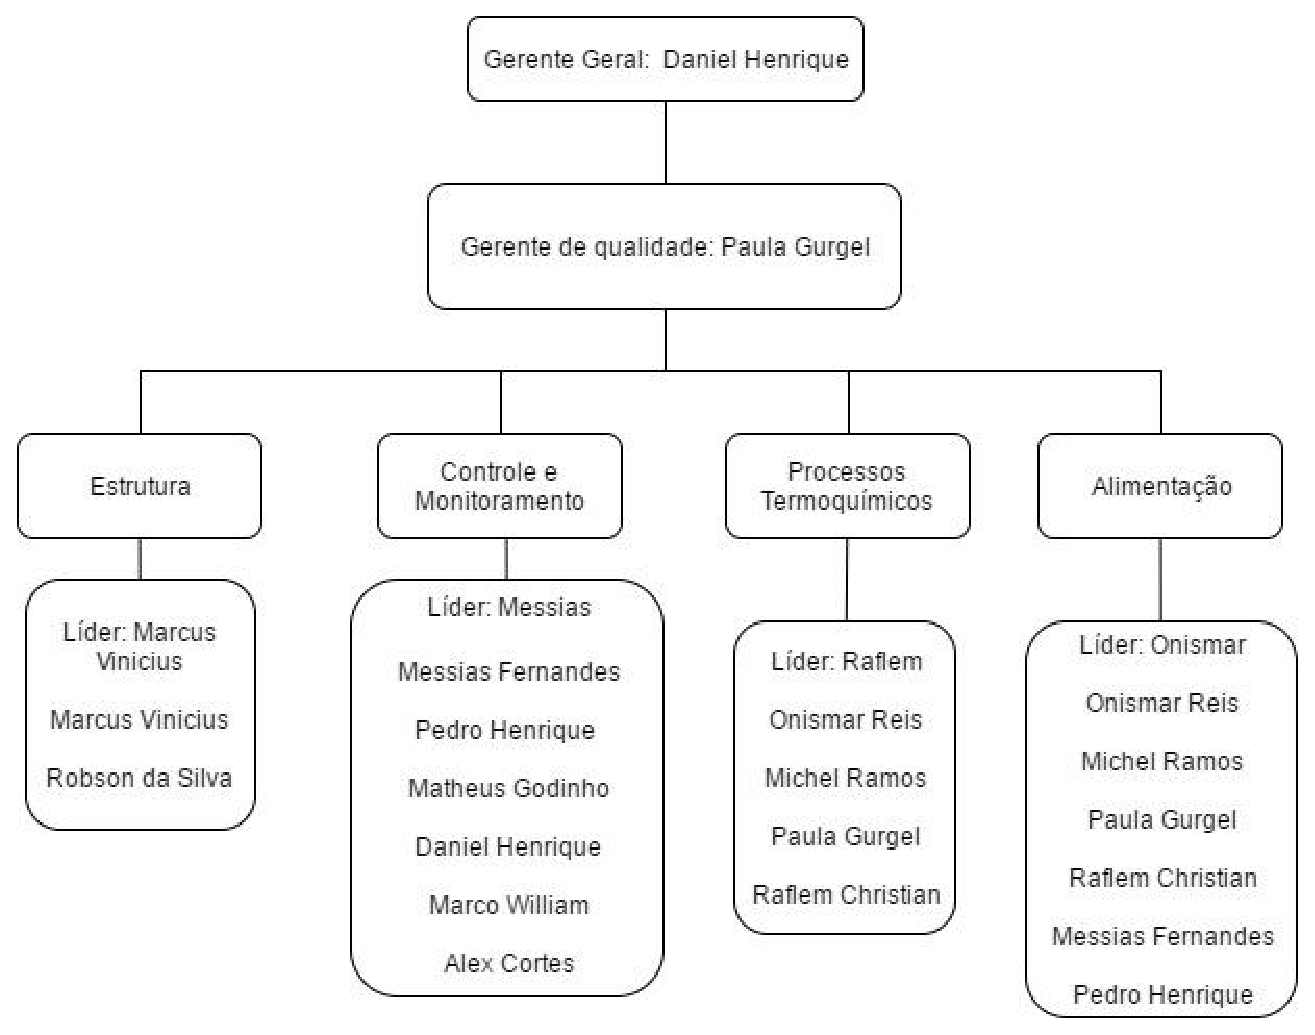
\includegraphics[keepaspectratio=true,scale=0.5]{figuras/divisao.eps}
	\caption{Divisão de frentes de trabalho e gerentes do projeto}
	\label{divisao}
\end{figure}

\subsection{Riscos}

Um plano de gerenciamento de riscos é necessário para calcular o impacto dos riscos no projeto e medidas de contingência para o controles dos mesmos. O plano de gerenciamento de riscos está disponível no anexo A.

\subsection{Requisitos}

A partir da concepção e validação do solucionamento do sistema, os requisitos foram definidos a partir de cada subsistema deste presente projeto.

\begin{itemize}
\item O biorreator deverá ser capaz de aquecer e resfriar dentro da faixa de 0º a 100º Celsius.
\item Ter um sistema que seja capaz de coletar CO2.
\item O rotor do sistema deverá manter-se a uma velocidade constante e pré-determinada.
\item O biorreator deverá possuir dimensões capazes de acomodar os sensores e demais componentes internos definidos no projeto.
\item Quanto a estrutura do biorreator, deverá possuir em sua composição, material favorável quanto a assepsia que o sistema necessita.
\item A dimensão da estrutura do biorreator deverá estar de conformidade com um equipamento de bancada de um laboratório.
\item O biorreator deverá possuir um motor, conectado ao seu rotor, para que a agitação mecânica seja realizada.
\item O biorreator deverá ser automatizado o suficiente para realizar a coleta de dados dos principais parâmetros e gerar gráficos.
\item O biorreator deverá realizar a leitura de dados referente a temperatura, pH, densidade e volume.
\item O biorreator deverá possuir um compartimento, especificamente de açúcar, para se auto-alimentar, quando necessário.
\item O biorreator deverá possuir uma válvula para realizar a coleta da levedura.
\item O biorreator deverá possuir uma válvula de precaução em caso de um aumento de pressão.
\item O biorreator deverá ter um sistema de aquecimento interligado a um controlador PID (Proporcional, Integral e derivativo).
\item Todo o sistema do biorreator deve estar conectado a um sistema de software e  hardware, que o usuário possa ver e controlar todos os parâmetros do mesmo.
\end{itemize}

\subsection{Controle e Monitoramento}

Dada a especificação do projeto, pretende-se realizar medições eletrônicas de valores de temperatura, densidade e potencial hidrogênico(pH). A partir, disso seria utilizado uma unidade microcontrolada para processamento de dados.

Com relação a unidade de controle e aquisição de dados para o monitoramento do sistema será atacado em duas frentes. A primeira solução adotada para este problema será usar uma \textit{Raspberry PI 3}, para realizar a aquisição e processamento de dados, para exercer essa atividade deve-se desenvolver uma biblioteca para cada sensor, com o auxílio de conversores analógicos/digitais para facilitar a recepção de dados pela Raspberry, essa solução pretende reduzir os itens envolvidos no projeto. Em paralelo será trabalhado uma solução alternativa, onde os dados enviados pelos sensores serão recebidos por um microcontrolador Arduino ATMEGA 238, e o dados serão processados e enviados para uma \textit{Raspberry PI 3}, através de um protocolo de comunicação \textit{UART}, para receber e realizar o processamento de dados.

\subsubsection{Medição de temperatura}

Para realizar medições de temperatura foi escolhido o sensor DS18B20, Com relação às suas especificações elétricas, este possui uma variação de tensão de alimentação nos seus pinos de -0.5 a +6V e a faixa de variação na escala de temperatura permite medições que variam de -55ºC a +125ºC. Esta escala de variação é adequada para a medição de valores de temperatura, já que o valor máximo para valores seria de aproximadamente 100ºC no interior do biorreator.

Sobre a precisão do componente, os valores de saída são discretizados na em 8 bits. Ou seja, os 180 valores possíveis de medição são exibidos com precisão de 0,703125ºC. O sensor além disso, possui características à prova de água, devido ao seu encapsulamento, o que facilita a imersão no interior do biorreator.

\begin{figure}[h]
	\centering
	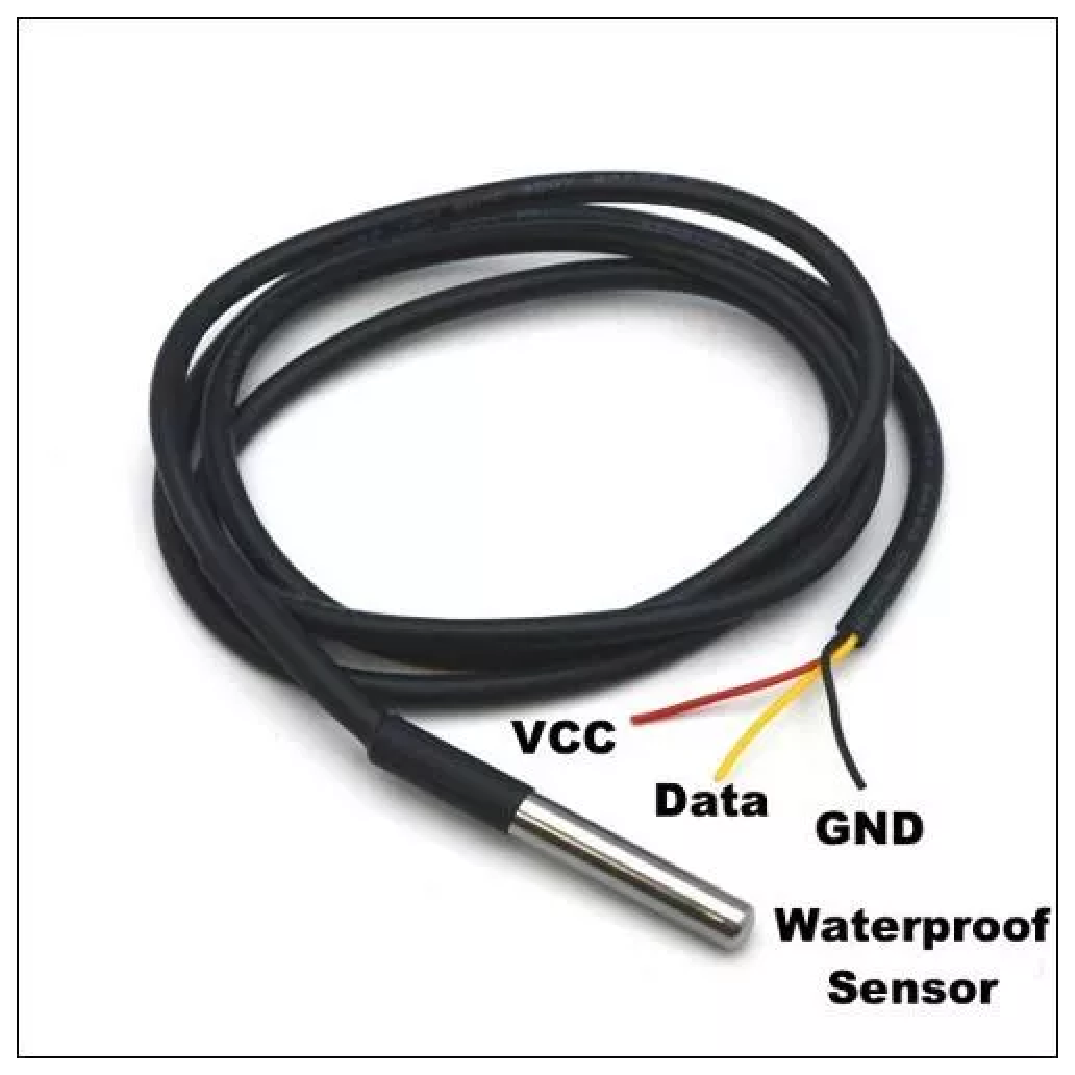
\includegraphics[keepaspectratio=true,scale=0.3]{figuras/probe.eps}
	\caption{Probe para imersão em fluidos}
	\label{probe}
\end{figure}

\subsubsection{Medição de densidade}

A definição da densidade no projeto é um requisito para provar a funcionalidade do projeto, torna-se necessário a sua medição. Considerando que o uso de um sensor de densidade é inviável de medição, usa-se o princípio da medição de pressão diferencial para estimar o valor da densidade através da manipulação da equação de Bernoulli. A especificação da medição de densidade, torna-se necessário o uso de sensores de pressão aplicados em dois pontos distintos no interior do biorreator.

\begin{figure}[h]
	\centering
	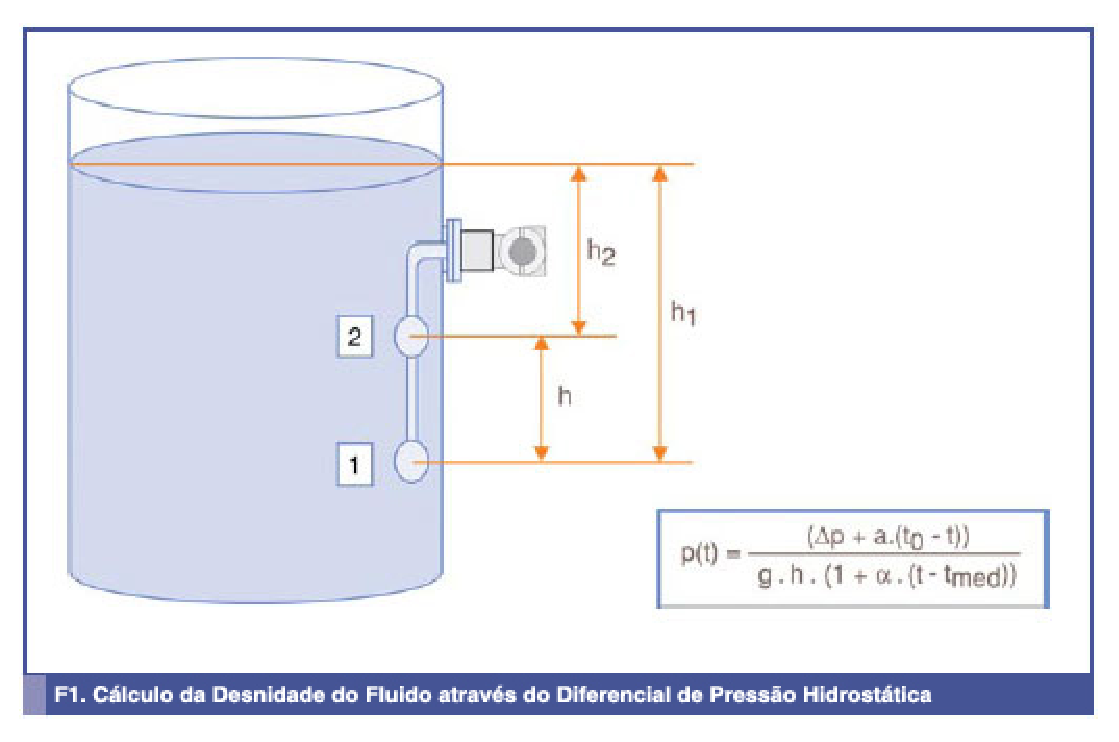
\includegraphics[keepaspectratio=true,scale=0.4]{figuras/densidade.eps}
	\caption{Modelo de cálculo da densidade de um fluido por pressão diferencial}
	\label{densidade}
\end{figure}

\subsubsection{Medição de Volume}

Tal componente utiliza sinais ultrassônicos para determinar a distância entre o sensor e um determinado obstáculo. De modo que no projeto em questão, será responsável por determinar a distância entre o sensor e o nível de açúcar presente na válvula, aferindo assim a quantidade de açúcar ali presente e retornando um dado para o servidor. Apresenta a seguinte tabela de especificações:

\begin{table}[h]
\centering
\caption{Especificações técnicas Sensor HC-SR04}
\resizebox{\textwidth}{!} {
\label{table2}
\begin{tabular}{|l|l|}
\hline
Tensão de Funcionamento                      & 5 V – DC                                              \\ \hline
Corrente de Funcionamento                    & 15 mA                                                 \\ \hline
Frequência de Funcionamento                  & 40 KHz                                                \\ \hline
Intervalo máximo de verificação de distância & 4 m                                                   \\ \hline
Intervalo mínimo de verificação de distância & 2 cm                                                  \\ \hline
ngulo de Detecção                            & 15º                                                   \\ \hline
Sinal de Entrada Trigger                     & 10uS pulso TTL                                        \\ \hline
Sinal de Saída Echo                          & Entrada do sinal de nível TTL e da faixa de proporção \\ \hline
Dimensão                                     & 45-20-15 mm                                           \\ \hline
\end{tabular}
}
\end{table}

\begin{figure}[h]
	\centering
	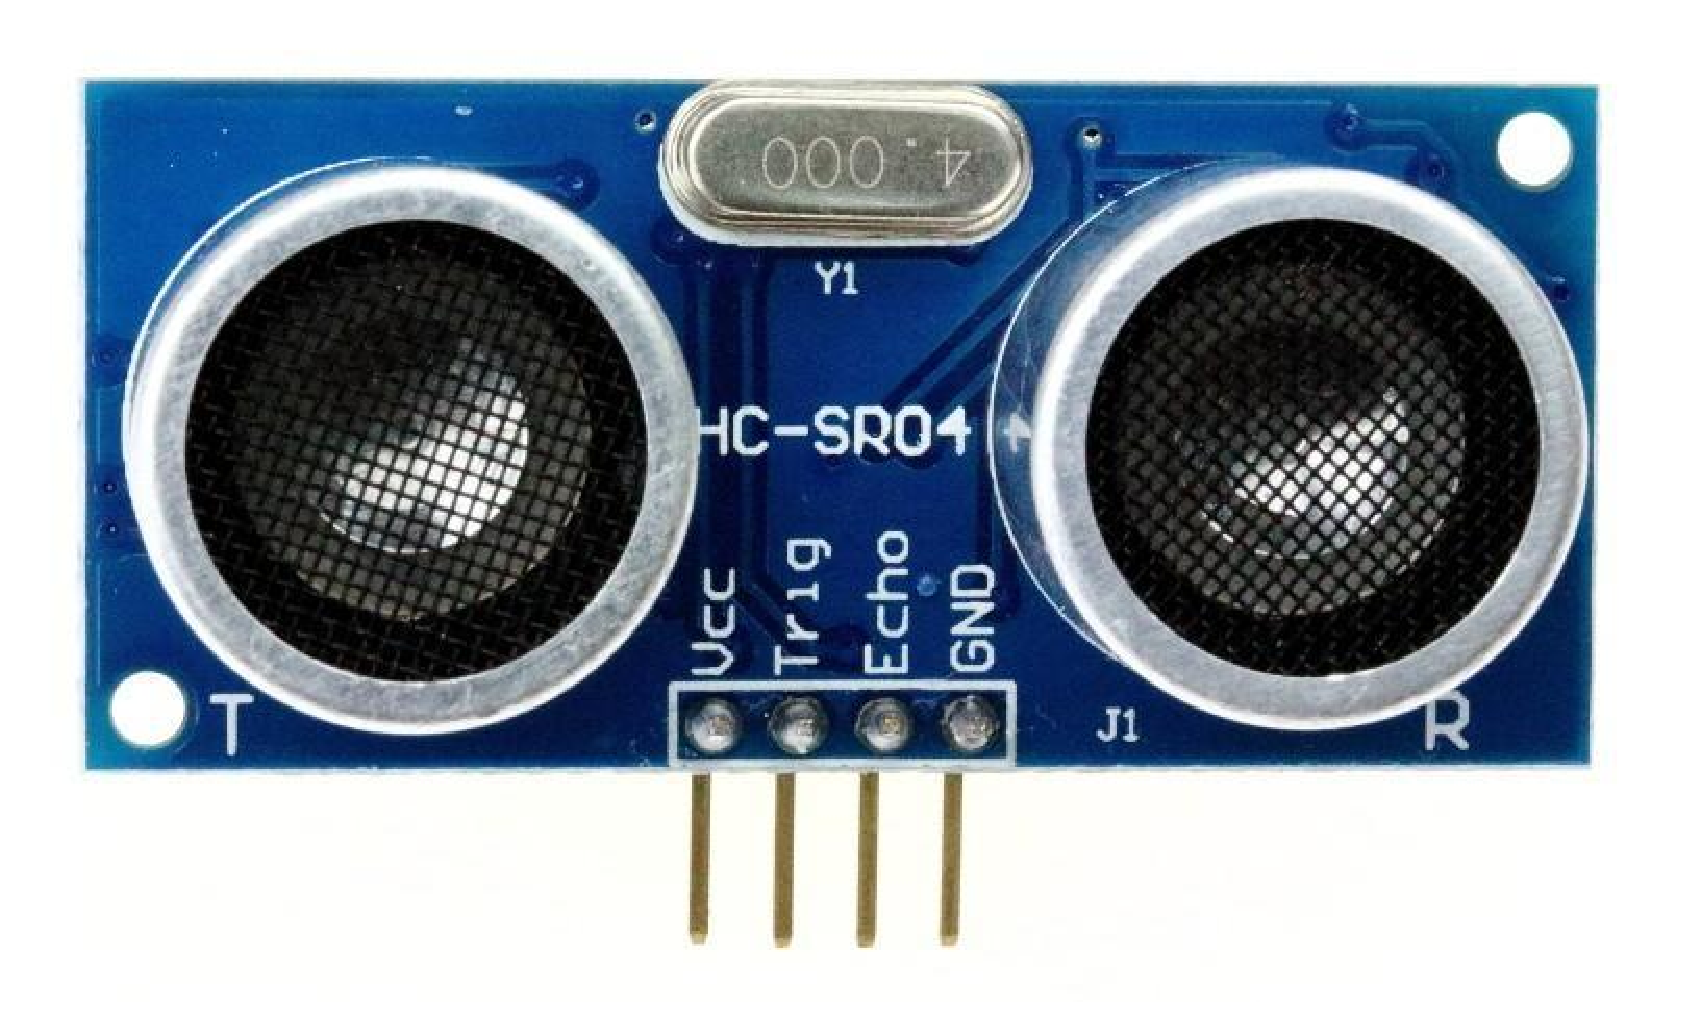
\includegraphics[keepaspectratio=true,scale=0.2]{figuras/sensor1.eps}
	\caption{Ilustração do Sensor HC-SR04}
	\label{sensor1}
\end{figure}

Assim como ilustrado pela imagem acima o componente possui 4 pinos (Vcc, Trigger, Echo, GND), onde serão conectados de acordo com as especificações técnicas ditas anteriormente.

\subsubsection{Medição de pH}

Com relação a especificação da medição de pH, torna-se necessário o uso do kit SKU: SEN0161 que é um kit integrado com um indicador de alimentação, um conector BNC e interface do sensor PH2.0. Segue abaixo a especificação:

\subsubsection{Válvula de Liberação de açúcar}

Para realizar a liberação de açúcar em tempos contínuos será utilizado um motor de passos para habilitar o despejo de açúcar na função de válvula. Para isso foi escolhido o componente Motor de Passo 28BYJ-48 + Driver ULN2003. Tal componente utiliza conversão de tensão em movimentos rotacionais, de modo a codificar o mesmo de modo a parar em posições específicas. De modo que este elemento será utilizado para o controle da válvula de depósito de açúcar, que quando acionado dá-se o passo necessário para liberação da quantidade de açúcar necessária para dentro do Biorreator. Já o Driver, é um sistema vendido juntamente ao motor, qual permite tal codificação de controle. Observa-se as seguintes especificações:

\begin{table}[h]
\centering
\caption{Especificação Motor de Passo 28BYJ-48}
\label{table3}
\begin{tabular}{|l|l|}
\hline
Tensão de Funcionamento & 5 V – DC   \\ \hline
Número de Fases         & 4          \\ \hline
Número de Vias          & 5          \\ \hline
Passos por Volta        & 64         \\ \hline
Torque máximo           & 2.2 Kgf.cm \\ \hline
Ângulo por passo        & 5.625º/64  \\ \hline
Frequência              & 100 Hz     \\ \hline
Diâmetro do Eixo        & 5 mm       \\ \hline
Peso                    & 40 g       \\ \hline
\end{tabular}
\end{table}

\begin{figure}[h]
	\centering
	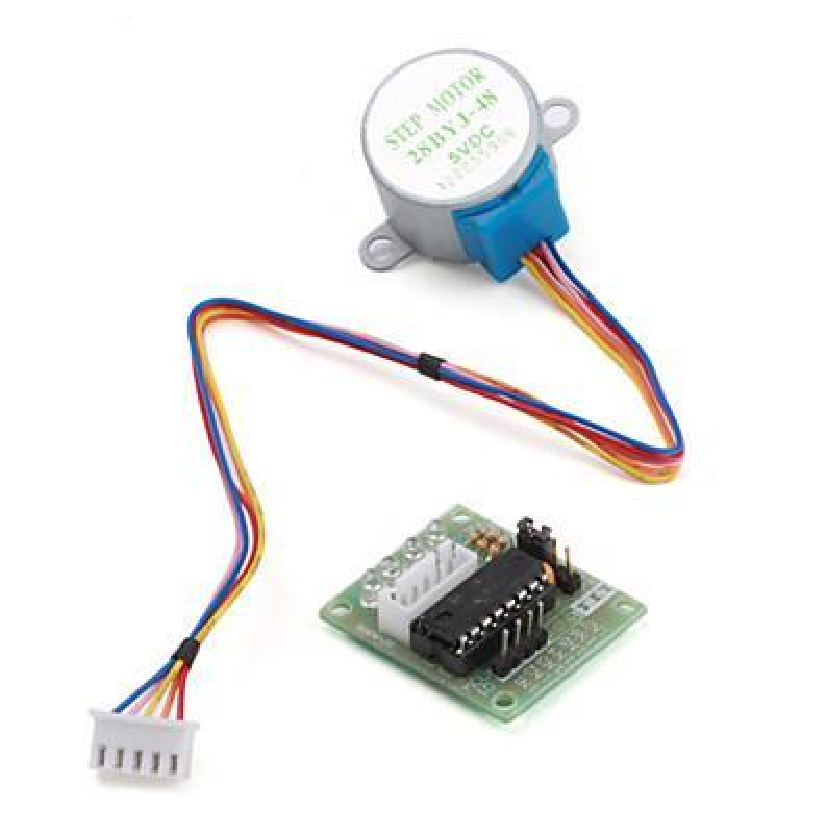
\includegraphics[keepaspectratio=true,scale=0.4]{figuras/sensor2.eps}
	\caption{Motor de Passo 28BYJ-48}
	\label{sensor2}
\end{figure}

\subsubsection{Conversor A/D ADS1115}

Tal componente realiza a conversão de tensão Analógica para Digital. Onde, na aplicação em estudo, será responsável por receber os sinais dos sensores em tensão analógica, converter para digital e encaminhar para o microcontrolador \textit{Raspberry}. Observa-se as seguintes especificações:

\begin{table}[h]
\centering
\caption{Especificações Conversor ADS1115}
\label{table4}
\begin{tabular}{|l|l|}
\hline
Tensão de Funcionamento    & 2.0 – 5.5 V (DC) \\ \hline
Canais                     & 4                \\ \hline
Resolução                  & 16 bits          \\ \hline
Frequência de operação SLC & 0.1 -3.4 MHz     \\ \hline
Taxa de Dados              & 8 – 860 SPS      \\ \hline
Dimensões                  & 2 x 1.5 x 0.4 mm \\ \hline
\end{tabular}
\end{table}

\begin{figure}[h]
	\centering
	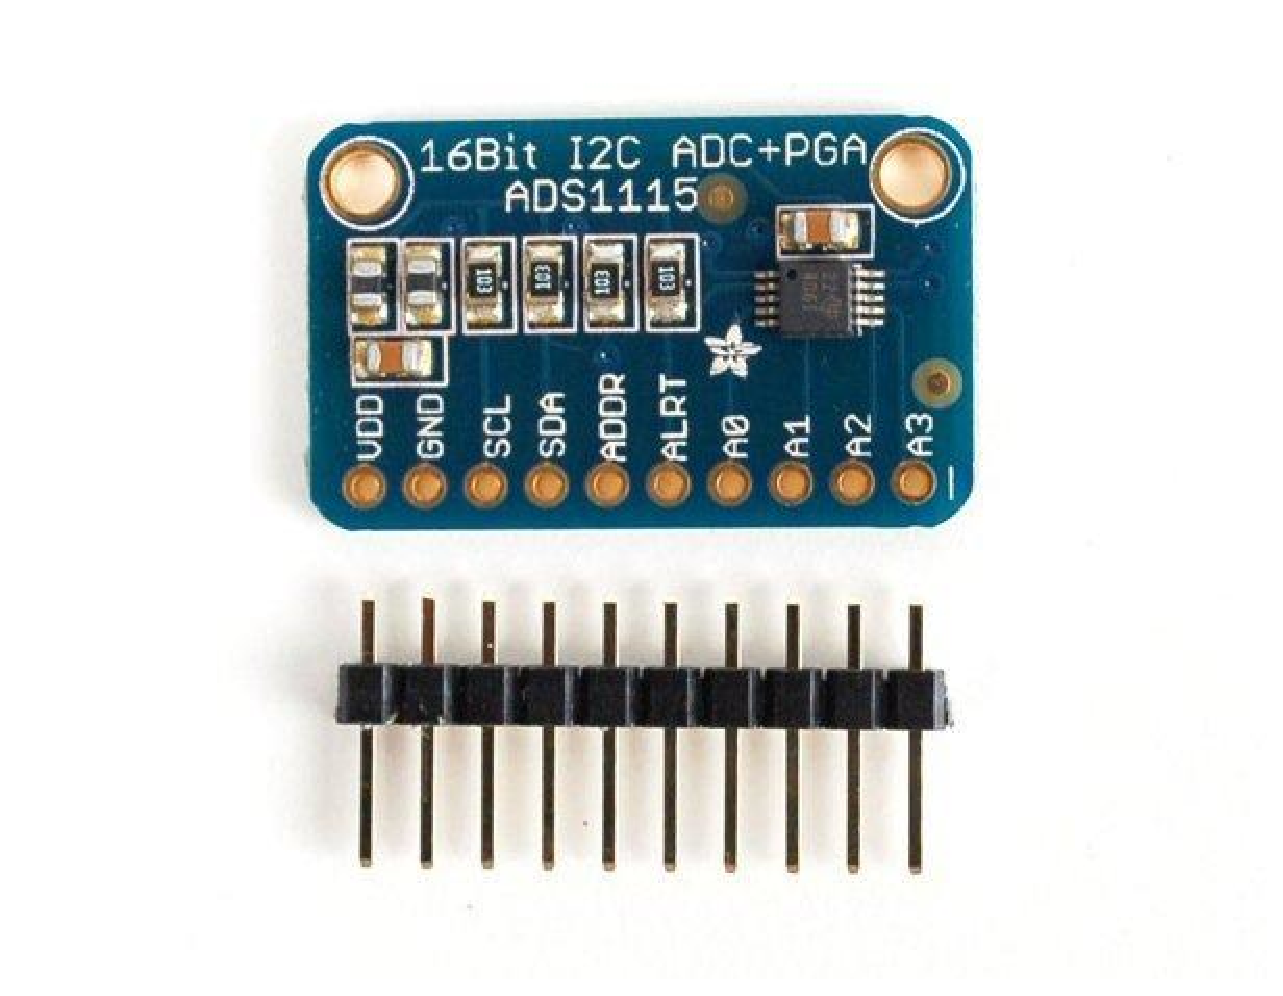
\includegraphics[keepaspectratio=true,scale=0.3]{figuras/sensor3.eps}
	\caption{Conversor ADS1115}
	\label{sensor3}
\end{figure}

\subsubsection{Conversor D/A MCP4725}

Tal componente realiza a conversão de tensão Digital para Analógico. Onde, na aplicação em estudo, será responsável por converter os sinais do cliente/usuário lançados pelo app em tensão digital, quais passam pelo servidor  microcontrolador \textit{Raspberry}, chegam no conversor em questão e são encaminhados para os Atuadores. Observa-se as seguintes especificações:

\begin{table}[h]
\centering
\caption{Especificações técnicas Conversor D/A MCP4725}
\label{table5}
\begin{tabular}{|l|l|}
\hline
Tensão de Funcionamento & 2.7 – 5.5 V (DC) \\ \hline
Canais                  & 1                \\ \hline
Resolução               & 12 bits          \\ \hline
\end{tabular}
\end{table}

\begin{figure}[h]
	\centering
	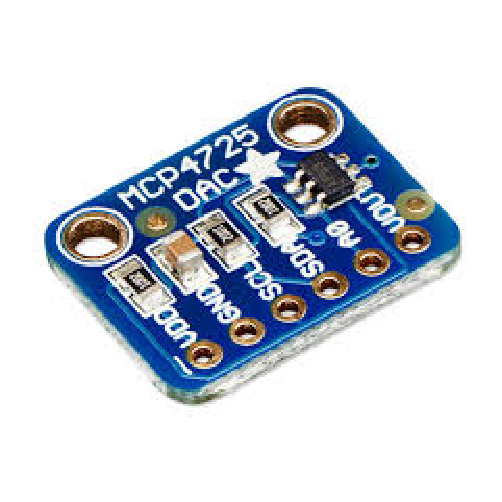
\includegraphics[keepaspectratio=true,scale=0.3]{figuras/sensor4.eps}
	\caption{Conversor D/A MCP4725}
	\label{sensor4}
\end{figure}

\subsubsection{Aplicativo}

Os requisitos do aplicativo foram definidos em formato de \textit{user stories}, identificadas como USXX sendo XX o número da \textit{user story}.

\subsubsubsection{US01}

Eu como usuário desejo visualizar os dados dos sensores para ter um monitoramento da fermentação no biorreator.

Critérios de aceitação:
\begin{itemize}
  \item Dados em forma de gráficos
  \item Gráficos gerados em tempo real
  \item Monitorar sensor de ph
  \item Monitorar sensor de densidade
  \item Monitorar sensor de temperatura
\end{itemize}

Tarefas:
\begin{itemize}
  \item Criar endpoint que disponibiliza os dados pela api
  \item Criar front-end no app para os gráficos
  \item Criar comunicação api-app para capturar os dados
\end{itemize}

\subsubsubsection{US02}

Eu como usuário desejo controlar a temperatura do biorreator para que a fermentação ocorra corretamente do início ao fim.

Critérios de aceitação:
\begin{itemize}
  \item Inserir a quantidade de graus desejada
\end{itemize}

Tarefas:
\begin{itemize}
  \item Criar endpoint para receber dados na api
  \item Criar front-end do app para receber a temperatura
  \item Criar comunicação app-api para enviar dados
\end{itemize

\subsubsubsection{US03}

Eu como usuário desejo criar uma fermentação para poder diferenciar os dados do aplicativo por fermentação

Critérios de aceitação:
\begin{itemize}
  \item Título
  \item Data de início
  \item Data de término
\end{itemize}

Tarefas:
\begin{itemize}
  \item Criar endpoint para salvar fermentação na api
  \item Criar front-end da criação de fermentação no app
  \item Criar comunicação app-api para salvar fermentação
\end{itemize}

\subsubsubsection{US04}
